
\subsection{Operational scenarios}
To study the different aspects of our predictions for the operation of the ITk strip system throughout its lifetime we performed the calculation of the system parameters over the expected 14 years of operation in monthly steps. Time-dependent inputs to the calculations were given from the expected performance of the LHC (figure~\ref{fig:opscenarios}a) and different profiles for the cooling temperature. We studied flat cooling temperature scenarios at different temperatures starting at -35$^\circ$C, the lowest evaporation temperature achievable with the ITk evaporative CO$_2$ cooling system, and a `ramp' scenario, where the cooling temperature starts at 0$^\circ$C and gradually is lowered down to -35$^\circ$C (figure~\ref{fig:opscenarios}b).

\begin{figure}[ht]
\centering
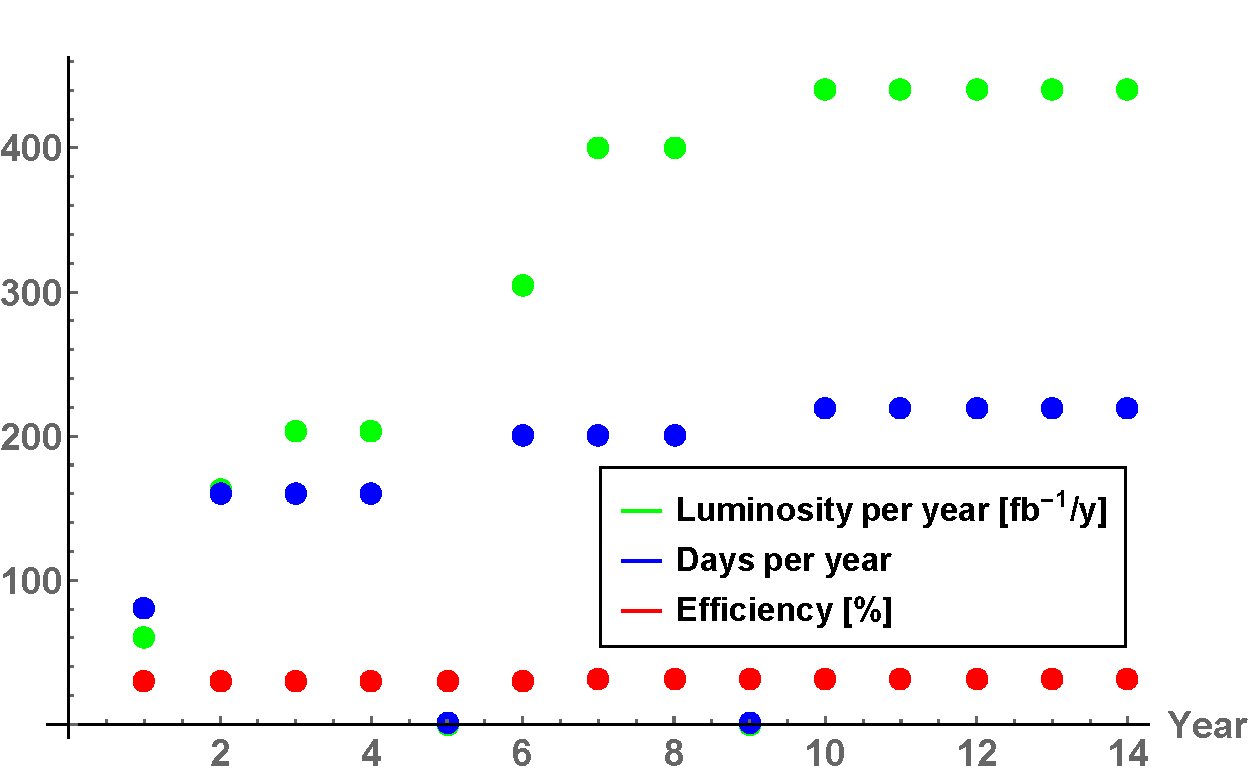
\includegraphics[width=0.4\linewidth]{figures/LHCperformance.pdf}\quad
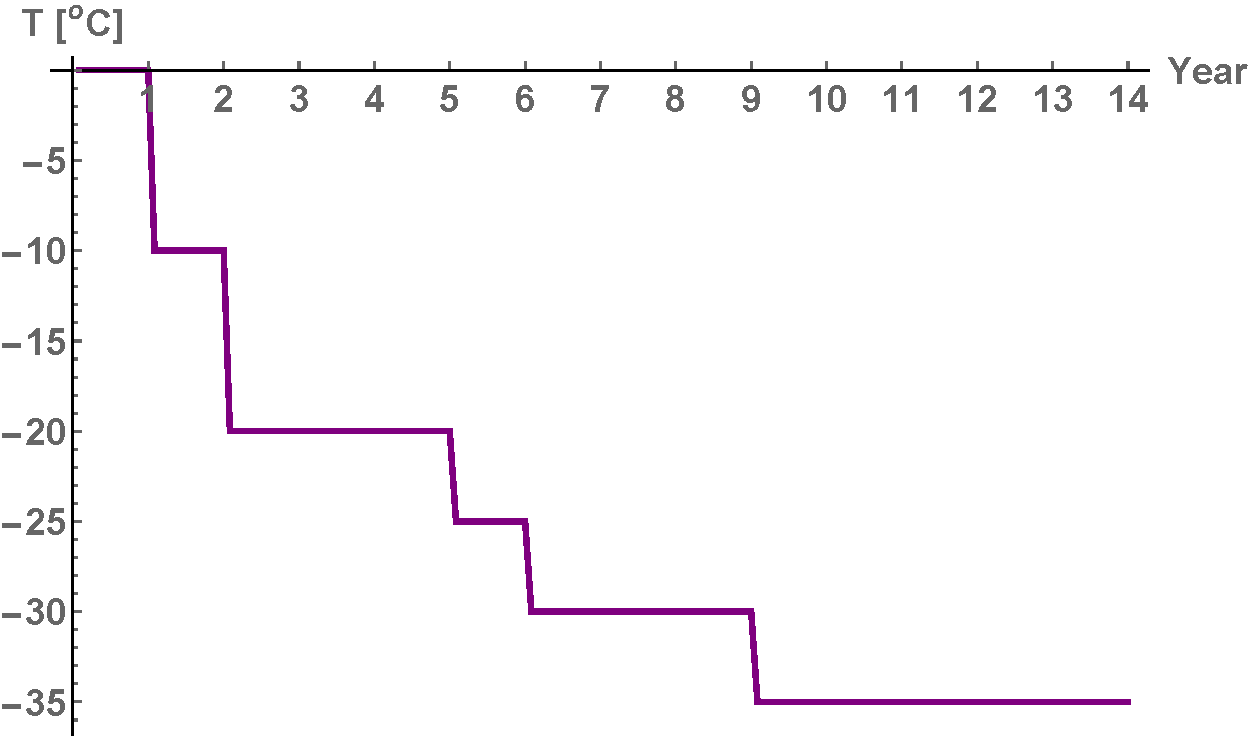
\includegraphics[width=0.4\linewidth]{figures/coolingramp.pdf}
\caption{Expected LHC performance (left) and cooling ramp' scenario for the cooling temperatures (right). Year-long shutdowns of the LHC are anticipated in years 5 and 9.}
\label{fig:opscenarios}
\end{figure}

\subsection{Safety factors}
To ensure the robustness of the system design against errors in the assumptions used in the model we ran the model in addition to the nominal set of input parameters with a set where some key inputs have been degraded. The set of safety factors used are given in table~\ref{tab:safetyfactors}. Each safety factor has been estimated individually based on experience, the complexity of the system aspect described by the parameter, and from available data or the absence of such data. Note that when the model was evaluated with safety factors all the safety factors in table~\ref{tab:safetyfactors} were used together, a situation which is unlikely to occur in the real system, thus providing a worst case estimate for the performance of the ITk strip system.

\begin{table}[htb]
\caption{Safety factors.}
\label{tab:safetyfactors}
\centering
\begin{tabular}{lcl}
Safety factor on & Value & Reason \\
\hline
Fluence  & 50\% & Accuracy of fluence calculations and uncertainties in material distributions\\
Thermal impedance & 10\% & Local support build tolerances\\
Digital current & 20\% & Final chip performance and parametrization of TID effect\\
Analog current & 5\% & Final chip performance\\
Tape impedance & 10\% & Electrical tape manufacturing tolerances\\
Bias voltage & 700~V & Increased bias voltage to maintain S/N\\
\end{tabular}
\end{table}

(Specifications using safety factor scenarios. Specifications for modules, global sytem requirements.
Qualitative understanding of system properties and evolution.)

